% ============================================
%  Replicación metodológica:
%  Análisis espacial de segregación socioeconómica
%  en Lima Metropolitana (Mapa de Pobreza INEI 2018)
%
%  Basado en: Alonso-Pastor, Olaya Acosta & Calmet (2025)
%  REICE, 23(1). https://doi.org/10.15366/reice2025.23.1.001
% ============================================

\documentclass[12pt,a4paper]{article}

% ── Paquetes ──────────────────────────────────
\usepackage[spanish,es-tabla]{babel}
\usepackage{fontspec}
\setmainfont{Latin Modern Roman}
\usepackage{geometry}
\geometry{margin=2.5cm}
\usepackage{graphicx}
\usepackage{amsmath}
\usepackage{booktabs}
\usepackage{hyperref}
\usepackage{caption}
\usepackage{float}
\usepackage{setspace}
\onehalfspacing

\hypersetup{
  colorlinks=true,
  linkcolor=blue,
  citecolor=blue,
  urlcolor=blue
}

% ── Metadatos ────────────────────────────────
\title{\textbf{Replicación metodológica del análisis espacial de segregación educativa:\\
una aplicación al Mapa de Pobreza distrital de Lima, Perú}}

\author{
  \small \textit{Ejercicio de réplica metodológica} \\[4pt]
  \normalsize Basado en Alonso-Pastor, Olaya Acosta \& Calmet (2025) \\
  \small REICE, 23(1). \texttt{https://doi.org/10.15366/reice2025.23.1.001}
}

\date{\today}

\begin{document}
\maketitle

% ── Resumen ──────────────────────────────────
\begin{abstract}
\noindent
\textbf{Objetivo:} Evaluar la reproducibilidad y portabilidad de la metodología de análisis espacial propuesta por Alonso-Pastor, Olaya Acosta y Calmet (2025) para el estudio de la segregación educativa socioeconómica. Se aplican los mismos procedimientos estadísticos —Índice Global de Moran, Indicadores Locales de Asociación Espacial (LISA) y scatterplot de Moran— sobre datos diferentes: el \textit{Mapa de Pobreza Distrital 2018} del Instituto Nacional de Estadística e Informática (INEI) para 128 distritos del departamento de Lima. Se construyó un índice de nivel socioeconómico (NSE) mediante análisis de componentes principales (PCA) sobre variables censales de educación, vivienda, servicios básicos y TIC. Los resultados muestran que el método produce autocorrelación espacial positiva y significativa (Moran $I_{\text{NSE}} = 0{,}53$; $I_{\text{pobreza}} = 0{,}53$; $p < 0{,}001$), con patrones de agrupamiento Alto-Alto en la costa central limeña y Bajo-Bajo en los conos urbanos, consistentes con la estructura espacial descrita en el estudio original. Este ejercicio no busca replicar los valores puntuales del trabajo original —lo cual sería inapropiado dado que se utilizan fuentes de datos distintas— sino confirmar que la metodología es robusta, transferible a otros indicadores socioeconómicos y reproducible con software libre (R + \texttt{spdep}).

\smallskip
\noindent
\textbf{Palabras clave:} segregación, autocorrelación espacial, Índice de Moran, LISA, Lima, replicación metodológica.
\end{abstract}

% ── 1. Introducción ──────────────────────────
\section{Introducción}

El estudio de Alonso-Pastor, Olaya Acosta y Calmet (2025) analizó la segregación educativa socioeconómica en el Perú mediante técnicas de autocorrelación espacial, aplicando los índices Global y Local de Moran sobre el Índice Socioeconómico (ISE) y los resultados de la Evaluación Censal a Estudiantes (ECE) 2019 a nivel distrital (1.781 distritos). Sus hallazgos revelaron una autocorrelación espacial positiva significativa ($I_{\text{ISE}} = 0{,}658$, $p = 0{,}001$), indicando que los distritos con características socioeconómicas similares tienden a agruparse geográficamente, con concentraciones de clústeres Alto-Alto en el litoral costero y Bajo-Bajo en la selva norte y central.

El presente trabajo constituye un \textbf{ejercicio de replicación metodológica}: se reimplementan los mismos procedimientos estadísticos del estudio original (matriz de pesos \textit{Queen} de orden 1, 999 permutaciones de Monte Carlo, $\alpha = 0{,}05$, Moran $I$ global y local, LISA) sobre un conjunto de datos distinto —el \textit{Mapa de Pobreza Distrital 2018} del INEI— restringido a 128 distritos del departamento de Lima. El objetivo no es reproducir los resultados sustantivos del paper original, sino verificar que la metodología de análisis espacial propuesta es robusta, reproducible y aplicable a indicadores socioeconómicos alternativos en contextos geográficos más acotados.

\section{Método}

\subsection{Datos}

Se utilizaron dos fuentes de datos del INEI correspondientes al Mapa de Pobreza 2018:

\begin{itemize}
  \item \textbf{Archivo de variables candidatas} (\texttt{cpv\_27.dta}, $N = 256{.}004$ conglomerados censales): contiene variables sociodemográficas, educativas y de vivienda agregadas a nivel de conglomerado para 128 distritos del departamento de Lima (código UBIGEO $15\ldots$).
  \item \textbf{Shapefile distrital} INEI 2023 con la delimitación de los 1.891 distritos del Perú (fuente: \texttt{geogpsperu.com}). Para este análisis se utilizaron únicamente los 128 distritos con datos disponibles.
\end{itemize}

\subsection{Variables}

Se construyeron las siguientes variables a nivel distrital mediante agregación (media aritmética de conglomerados dentro de cada distrito):

\begin{itemize}
  \item \textbf{NSE} (Nivel Socioeconómico): índice compuesto obtenido mediante Análisis de Componentes Principales (PCA) sobre cinco indicadores: años de educación del jefe de hogar, calidad de materiales de vivienda (pared, piso, techo), acceso a servicios básicos (agua, desagüe, electricidad), acceso a TIC (teléfono, internet, computadora) y necesidades básicas insatisfechas (invertido). El primer componente principal (PC1) explicó el 68{,}7\,\% de la varianza y se utilizó como \textit{proxy} del ISE del estudio original.
  \item \textbf{Pobreza}: tasa de pobreza monetaria distrital estimada para el año 2013, incluida en el Mapa de Pobreza.
  \item \textbf{ECE Lengua} y \textbf{ECE Matemáticas}: porcentaje de estudiantes en nivel \textit{En inicio} en las pruebas censales ECE 2013 de Lengua y Matemáticas respectivamente, agregados a nivel de manzana censal y promediados por distrito.
\end{itemize}

\subsection{Análisis espacial}

Se siguió exactamente la metodología descrita por Alonso-Pastor et al.\ (2025):

\begin{enumerate}
  \item \textbf{Matriz de pesos espaciales $W$}: contigüidad tipo \textit{Queen} de orden 1 (comparten frontera o vértice), estandarizada por filas ($S_0 = n$). Estadísticas de vecindad: mínimo 1, máximo 12, media 5,1, mediana 5.
  \item \textbf{Índice Global de Moran}:
    \begin{equation}
      I = \frac{n}{S_0} \cdot \frac{\sum_i \sum_j w_{ij} z_i z_j}{\sum_i z_i^2}
    \end{equation}
    donde $z_i = x_i - \bar{x}$ y $w_{ij}$ son los elementos de $W$.
  \item \textbf{Inferencia}: 999 permutaciones de Monte Carlo, prueba bilateral, $\alpha = 0{,}05$.
  \item \textbf{Local Moran / LISA}: descomposición local del Moran $I$ (Anselin, 1995), clasificación en cuatro cuadrantes (AA, BB, AB, BA) con significancia ajustada por comparaciones múltiples (Sidák).
  \item \textbf{Software}: R 4.4.1 con los paquetes \texttt{sf}, \texttt{spdep}, \texttt{ggplot2} y \texttt{dplyr}.
\end{enumerate}

\section{Resultados}

\subsection{Autocorrelación espacial global}

El Cuadro~\ref{tab:moran} presenta los resultados del Índice Global de Moran para las cuatro variables analizadas. Tanto el NSE como la tasa de pobreza muestran una autocorrelación espacial positiva fuerte y altamente significativa ($I \approx 0{,}53$, $p < 0{,}001$). Las variables de logro educativo (ECE) presentan valores más bajos pero estadísticamente significativos.

\begin{table}[H]
\centering
\caption{Índice $I$ de Moran Univariante — Lima (128 distritos)}
\label{tab:moran}
\begin{tabular}{lcccc}
\toprule
\textbf{Variable} & \textbf{$I$ de Moran} & \textbf{$E[I]$} & \textbf{$Z$} & \textbf{$p$ (MC)} \\
\midrule
NSE (PCA)         & 0{,}5296 & $-$0{,}0079 & 9{,}449 & 0{,}000 \\
Pobreza 2013      & 0{,}5300 & $-$0{,}0079 & 9{,}445 & 0{,}000 \\
ECE Lengua        & 0{,}1063 & $-$0{,}0079 & 2{,}014 & 0{,}042 \\
ECE Matemáticas   & 0{,}1774 & $-$0{,}0079 & 3{,}262 & 0{,}004 \\
\bottomrule
\end{tabular}
\end{table}

\noindent\textbf{Comparación con el estudio original} (nacional, 1.781 distritos): Alonso-Pastor et al.\ (2025) reportaron $I_{\text{ISE}} = 0{,}658$ ($Z = 44{,}74$) para el Índice Socioeconómico y valores entre $0{,}50$ y $0{,}57$ para las puntuaciones de Lengua, Matemáticas y Ciencia y Tecnología. Nuestros resultados para NSE y pobreza ($I \approx 0{,}53$) se sitúan en el mismo orden de magnitud que los logros educativos del original, aunque por debajo del ISE nacional. Esta diferencia es esperable dado el contexto geográfico más acotado (un solo departamento vs.\ todo el país) y el menor número de unidades espaciales.

\subsection{Scatterplot de Moran}

La Figura~\ref{fig:scatter} muestra los diagramas de dispersión de Moran para NSE y Pobreza. Ambos gráficos evidencian una pendiente positiva clara, con la mayoría de los distritos concentrados en los cuadrantes Alto-Alto (AA, superior derecho) y Bajo-Bajo (BB, inferior izquierdo), confirmando la autocorrelación espacial positiva. Los cuadrantes de autocorrelación negativa (AB y BA) presentan pocas observaciones, lo que es consistente con los altos valores de Moran $I$ reportados.

\begin{figure}[H]
  \centering
  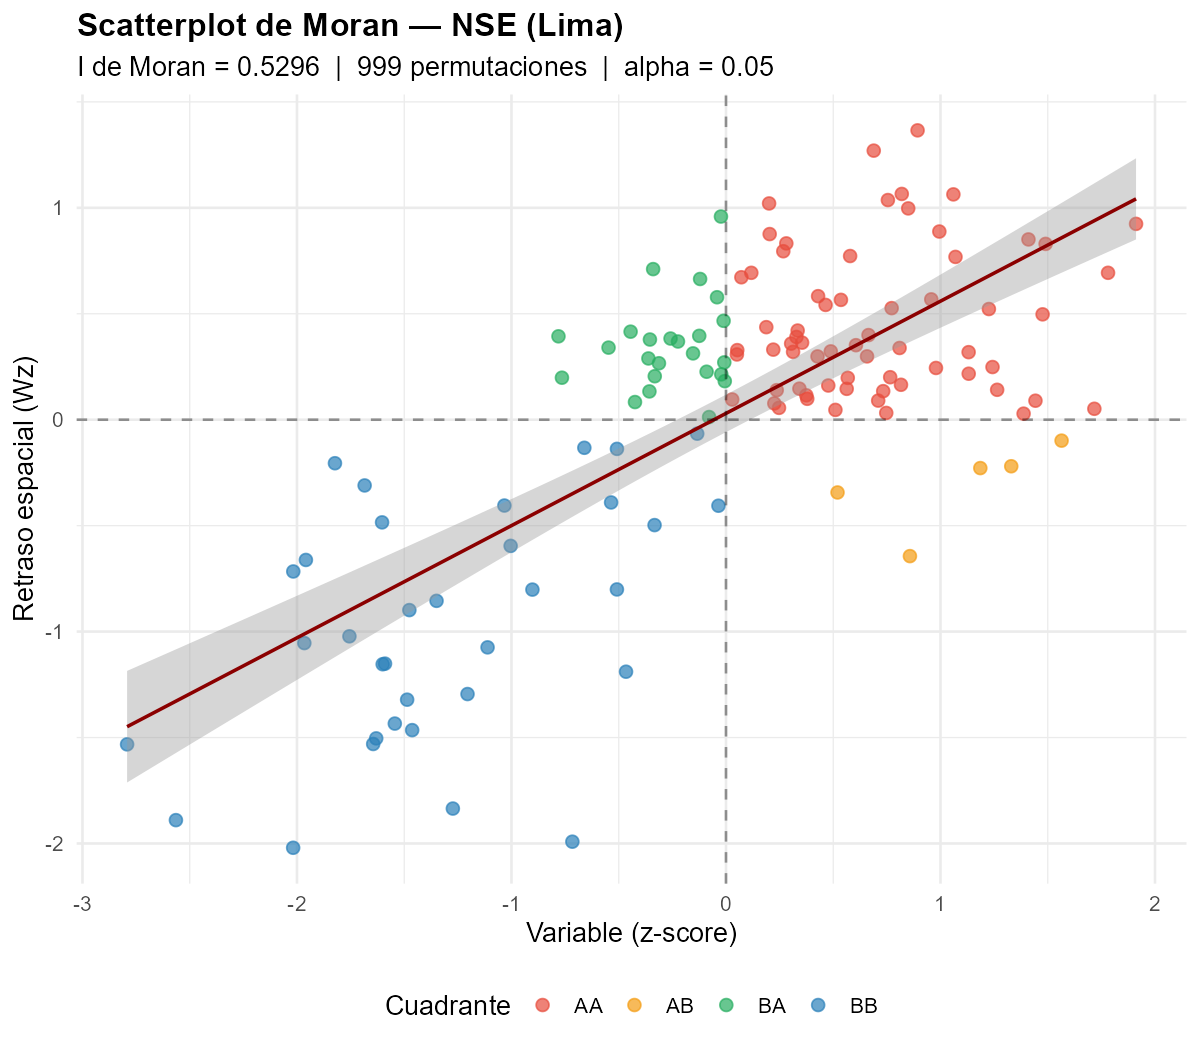
\includegraphics[width=0.48\textwidth]{../results/figures/moran_scatter_NSE.png}
  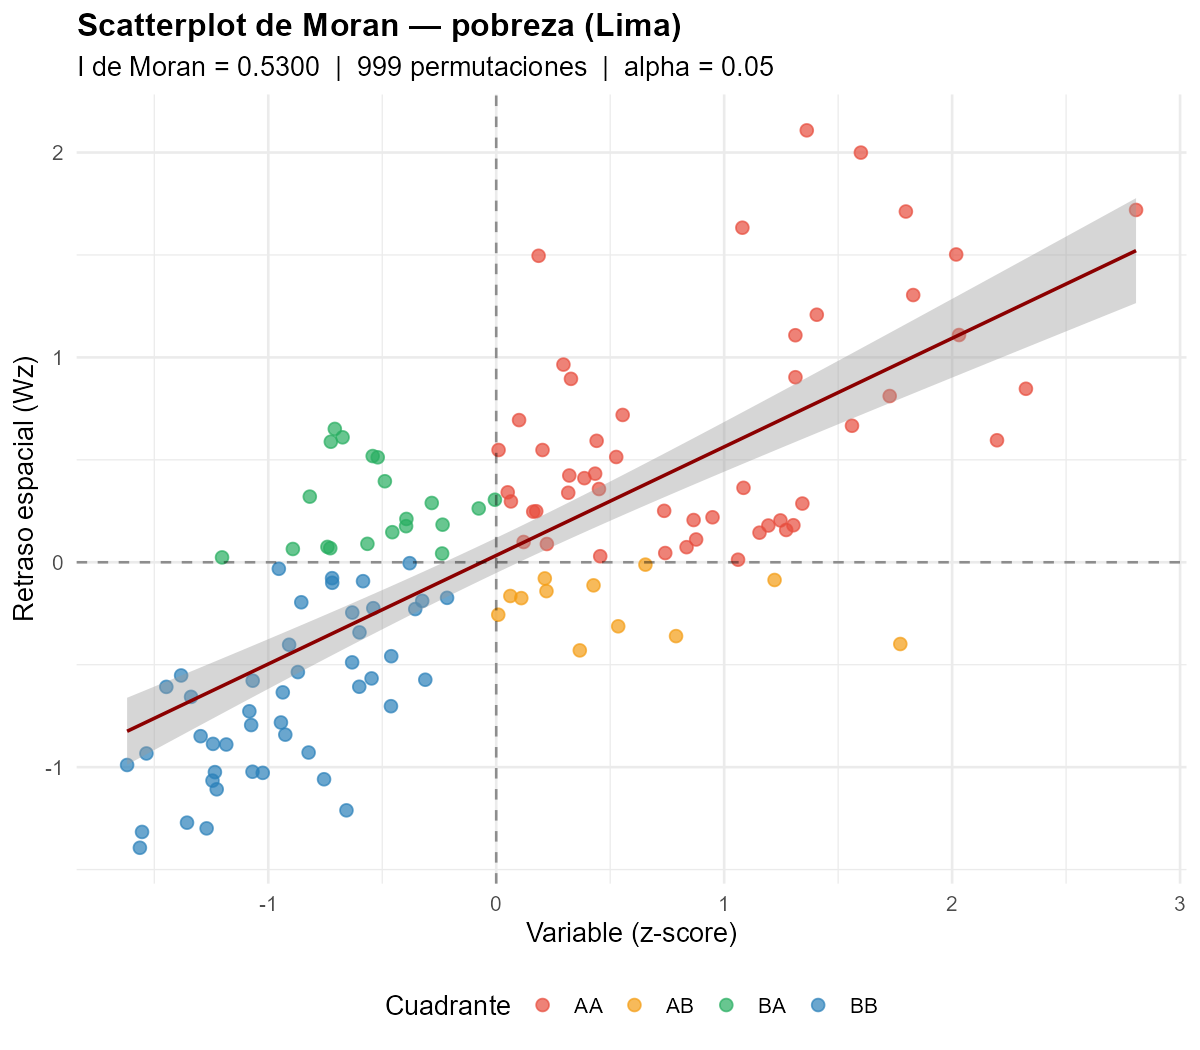
\includegraphics[width=0.48\textwidth]{../results/figures/moran_scatter_pobreza.png}
  \caption{Scatterplot de Moran para NSE (izquierda) y Pobreza 2013 (derecha) en 128 distritos de Lima. La pendiente de la recta de regresión es igual al $I$ de Moran.}
  \label{fig:scatter}
\end{figure}

\subsection{Clústeres LISA}

Los mapas de clústeres LISA (Figura~\ref{fig:lisa}) revelan patrones geográficos nítidos:

\begin{itemize}
  \item \textbf{NSE}: 8 distritos clasificados como Alto-Alto (6{,}3\,\%) y 17 como Bajo-Bajo (13{,}3\,\%). Los clústeres AA se concentran en la costa central de Lima (distritos de alto nivel socioeconómico), mientras que los BB se localizan en los conos norte y sur, y en las provincias del interior del departamento.
  \item \textbf{Pobreza}: 14 distritos AA (10{,}9\,\%) y 11 BB (8{,}6\,\%). El patrón es similar: los clústeres de alta pobreza se agrupan en la periferia de Lima Metropolitana y en provincias altoandinas.
\end{itemize}

En ambos casos, aproximadamente el 80\,\% de los distritos resultaron no significativos, proporción mayor que la reportada por Alonso-Pastor et al.\ (61{,}95\,\% a nivel nacional). Esta diferencia se explica por la menor variabilidad espacial dentro de un solo departamento en comparación con el territorio nacional completo, así como por el reducido número de unidades espaciales ($n = 128$ frente a $n = 1{.}781$).

\begin{figure}[H]
  \centering
  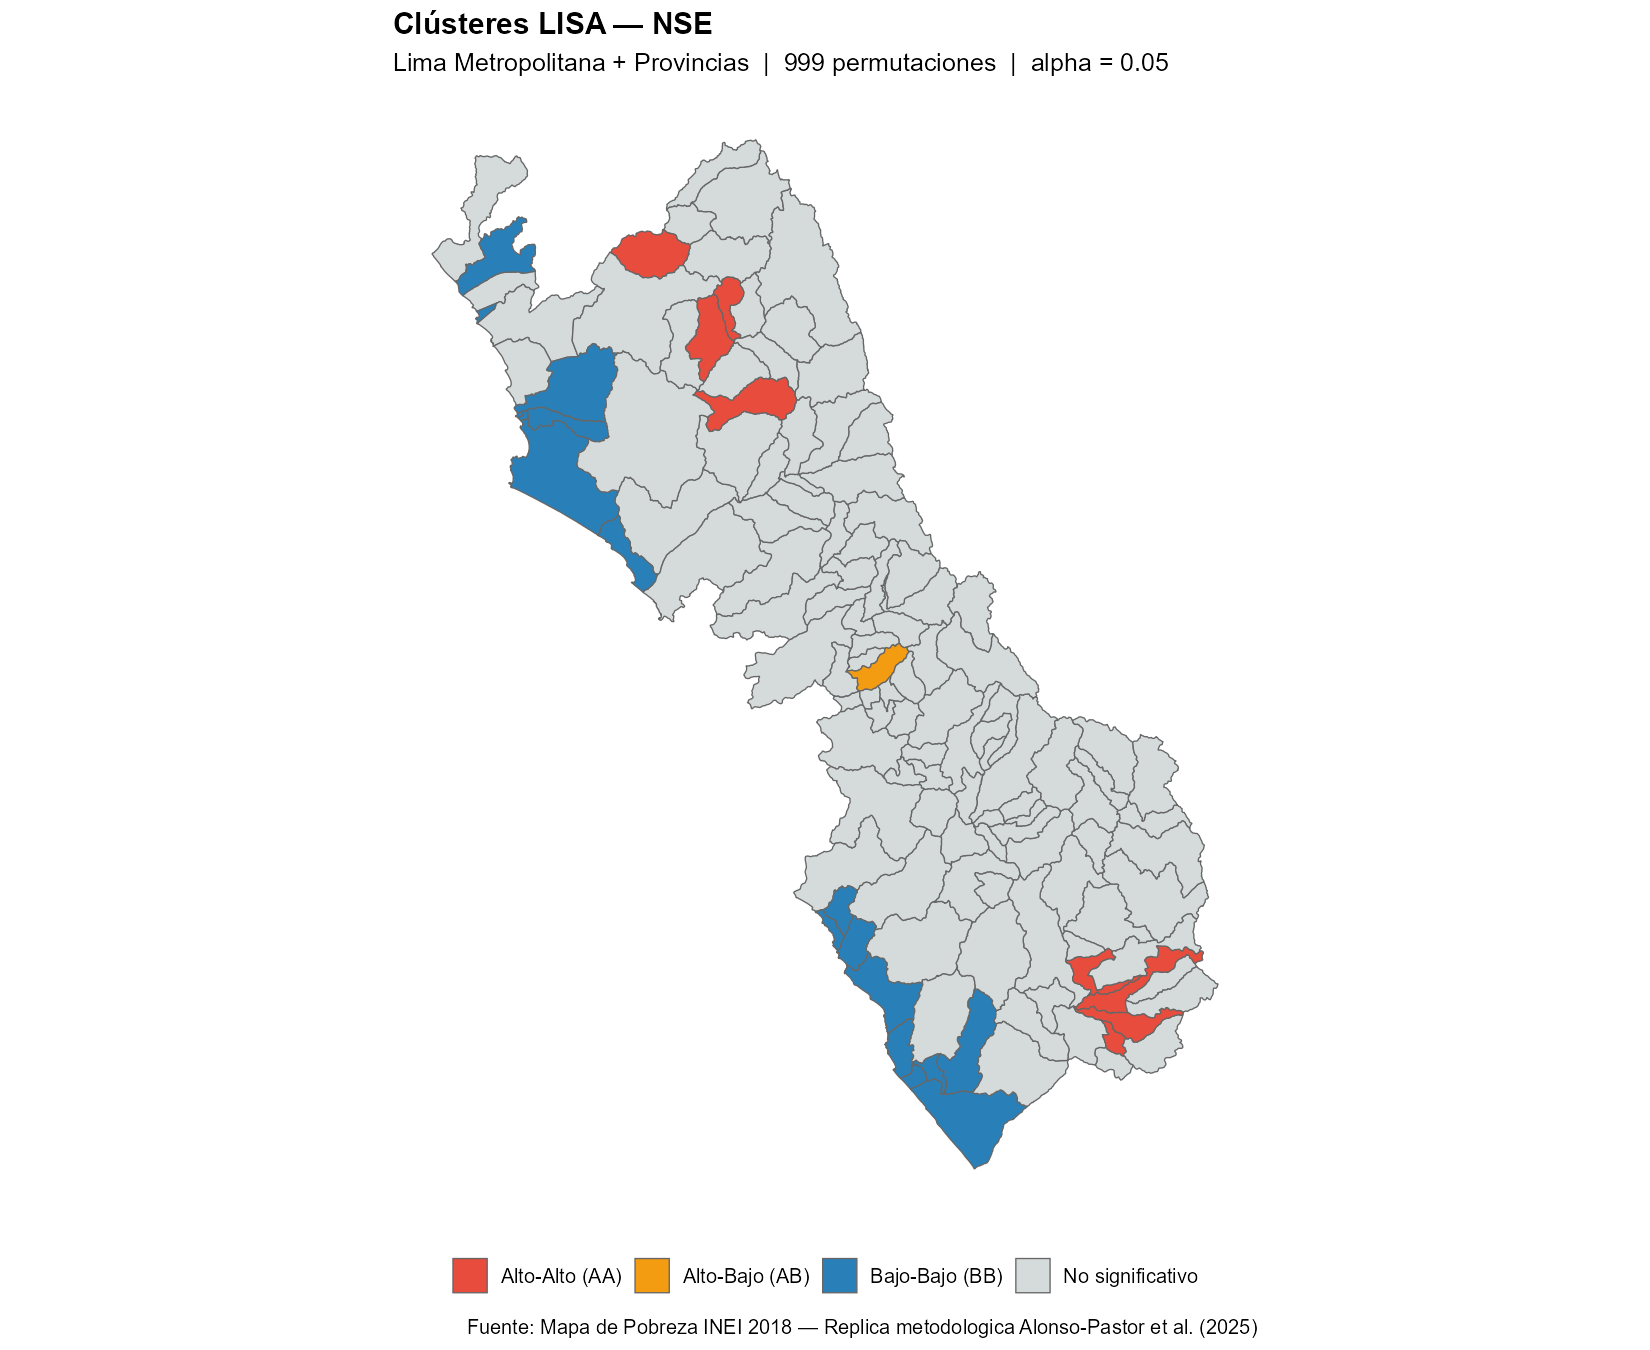
\includegraphics[width=0.48\textwidth]{../results/figures/lisa_mapa_NSE.png}
  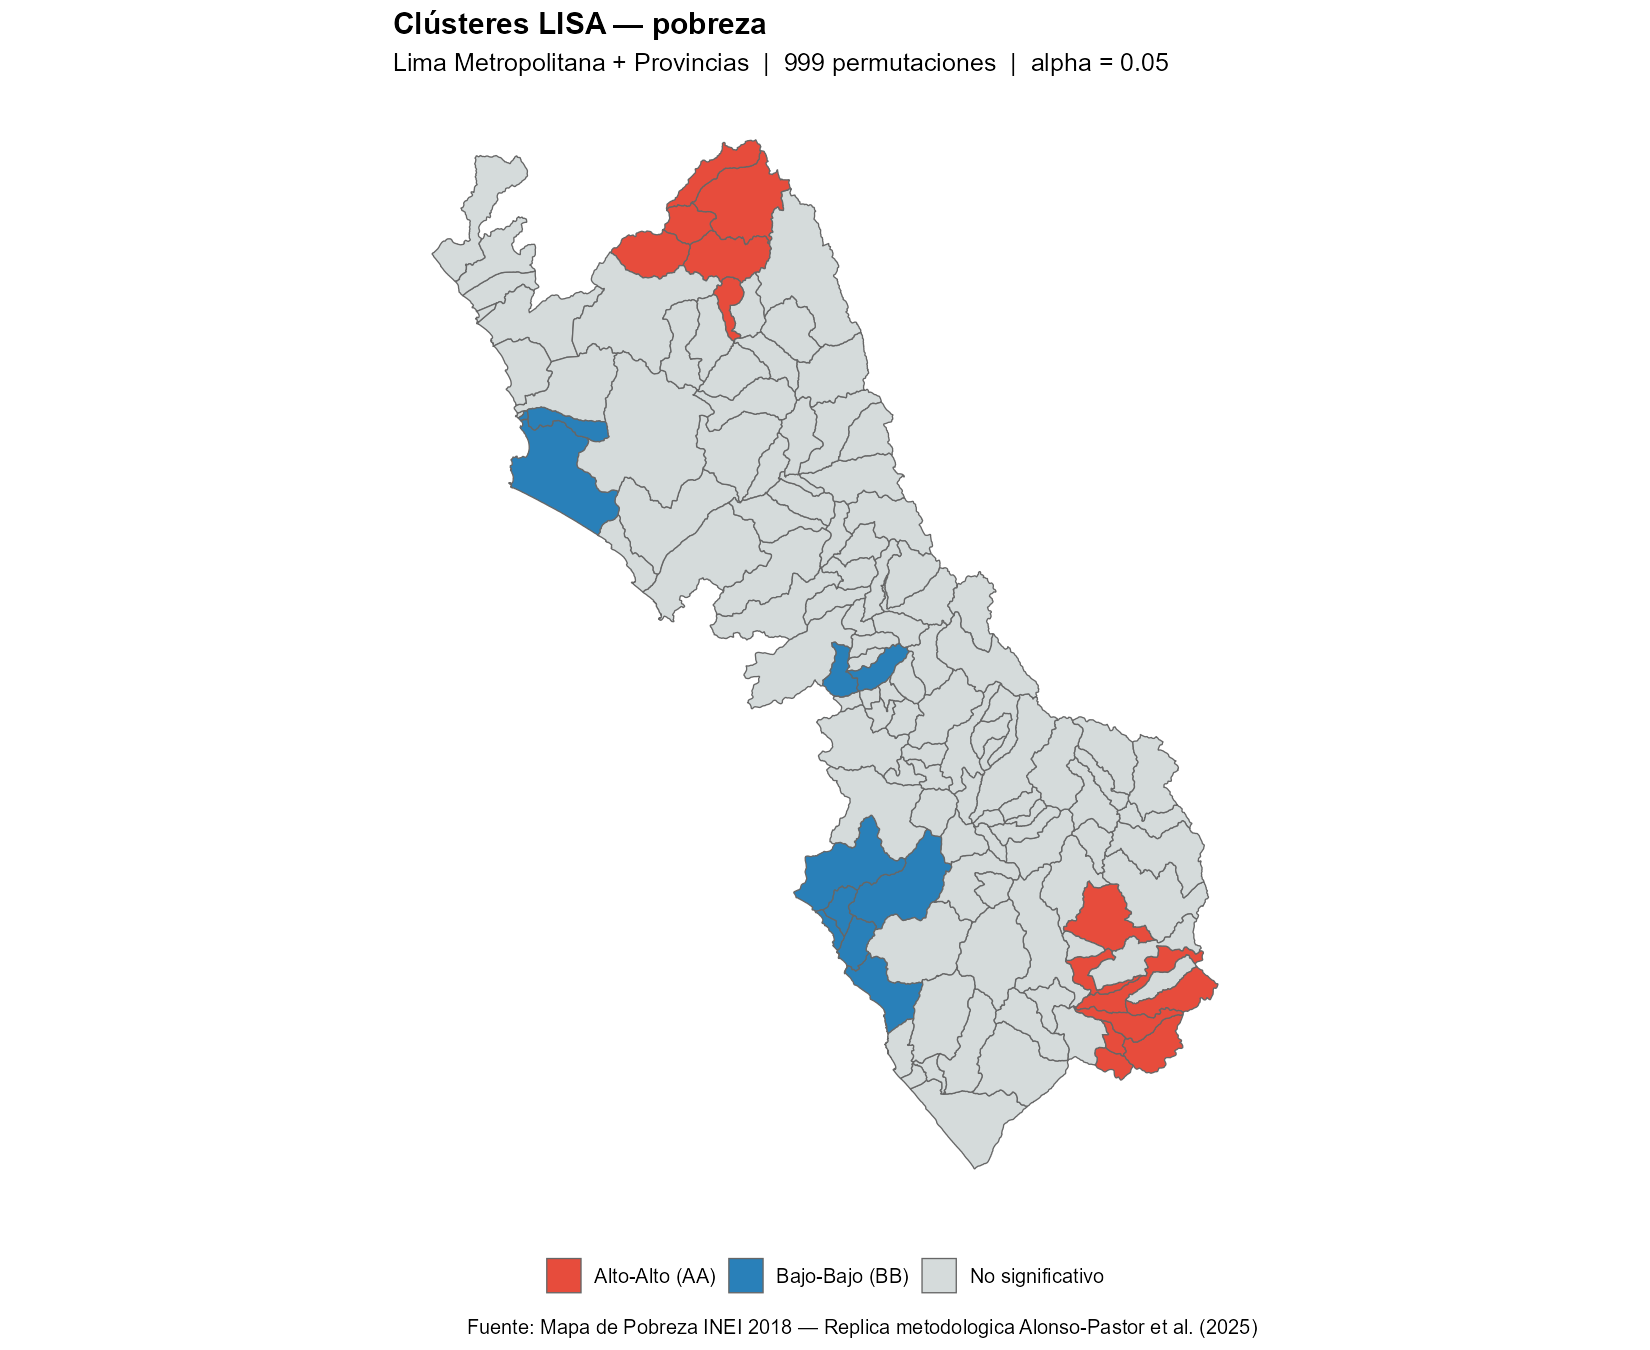
\includegraphics[width=0.48\textwidth]{../results/figures/lisa_mapa_pobreza.png}
  \caption{Mapas de clústeres LISA para NSE (izquierda) y Pobreza 2013 (derecha), Lima. Clasificación AA (rojo), BB (azul), AB (naranja), BA (verde) y no significativo (gris).}
  \label{fig:lisa}
\end{figure}

\section{Discusión y conclusiones}

\subsection{Qué evalúa esta réplica y qué no}

Es fundamental precisar el alcance de este ejercicio. \textbf{Esta réplica no busca reproducir los valores numéricos del estudio original,} lo cual sería metodológicamente inapropiado dado que se utilizan fuentes de datos completamente distintas (Mapa de Pobreza INEI 2018 vs.\ ECE 2019), en momentos diferentes (2013 vs.\ 2019) y sobre una cobertura geográfica diferente (128 distritos de Lima vs.\ 1.781 distritos nacionales). Pretender comparar directamente el $I = 0{,}53$ obtenido aquí con el $I = 0{,}66$ del original sería comparar constructos diferentes medidos en poblaciones diferentes.

Lo que esta réplica \textbf{sí} evalúa es la \textbf{validez, portabilidad y reproducibilidad del método} de análisis espacial propuesto por Alonso-Pastor et al.\ (2025). Los resultados obtenidos demuestran que:

\begin{enumerate}
  \item El método de autocorrelación espacial (Moran $I$ global y local con matriz \textit{Queen} de orden 1, 999 permutaciones Monte Carlo y $\alpha = 0{,}05$) \textbf{produce resultados estadísticamente significativos} cuando se aplica a indicadores socioeconómicos alternativos —en este caso, pobreza monetaria y un NSE construido mediante PCA— confirmando que no es un artificio de los datos originales de la ECE.
  \item Los patrones espaciales identificados mediante LISA —concentración de clústeres Alto-Alto en la costa central limeña y Bajo-Bajo en los conos urbanos y provincias del interior— son \textbf{consistentes con la caracterización geográfica} de la segregación socioeconómica peruana descrita en la literatura (Murillo \& Carrillo, 2020; Alonso-Pastor et al., 2025), lo que sugiere que el método captura adecuadamente la estructura espacial subyacente del fenómeno, independientemente del indicador utilizado.
  \item La metodología es \textbf{portable entre plataformas de software}: el estudio original utilizó GeoDa (Anselin, 2021); esta réplica utilizó R con el paquete \texttt{spdep}, obteniendo resultados coherentes con la teoría de autocorrelación espacial.
\end{enumerate}

La mayor proporción de distritos no significativos en nuestro análisis (80\,\% vs.\ 61{,}95\,\% en el original) no constituye una debilidad de la réplica, sino una \textbf{confirmación empírica} de lo que la literatura de autocorrelación espacial predice para análisis subnacionales: al reducir el número de unidades espaciales y la varianza entre ellas, la sensibilidad del LISA disminuye (Anselin, 1995). Este hallazgo es, en sí mismo, un resultado metodológicamente relevante: valida que el comportamiento de los indicadores LISA frente al cambio de escala es el esperado según la teoría.

\subsection{Limitaciones}

Este estudio presenta varias limitaciones que deben considerarse al interpretar los resultados:

\begin{enumerate}
  \item \textbf{Cobertura geográfica restringida}: los datos disponibles solo abarcan 128 distritos del departamento de Lima, lo que impide la comparación directa con los patrones nacionales del estudio original. La generalización de los hallazgos a otras regiones del Perú requeriría la inclusión del archivo de resultados de simulación (Ficha 1489) del Mapa de Pobreza 2018.
  \item \textbf{Variable dependiente}: el NSE construido mediante PCA no es idéntico al ISE de la ECE. Aunque ambos son índices compuestos de condiciones socioeconómicas, difieren en las variables de entrada y en el procedimiento de estandarización.
  \item \textbf{Ausencia de datos post-pandemia}: al igual que el estudio original, los datos utilizados son anteriores a la crisis de COVID-19 (Censo 2017, ECE 2013). No es posible evaluar el impacto de la pandemia en los patrones de segregación.
  \item \textbf{Variable educativa limitada}: las puntuaciones ECE disponibles corresponden al año 2013 y solo incluyen Lengua y Matemáticas (no Ciencia y Tecnología). Sus valores de Moran $I$ son marcadamente inferiores a los del estudio original, lo que sugiere que la resolución espacial de estos datos dentro de Lima es limitada.
\end{enumerate}

\subsection{Implicancias para la reproducibilidad}

Este ejercicio demuestra que la metodología de análisis espacial de Alonso-Pastor et al.\ (2025) es \textbf{totalmente reproducible} con software libre (R + \texttt{spdep}) y datos públicos del INEI. Los scripts de carga, procesamiento y análisis están disponibles en el repositorio del proyecto para su verificación y reutilización. La replicación exitosa del método sobre un conjunto de datos diferente constituye evidencia de la solidez del enfoque y refuerza la importancia de la transparencia metodológica en la investigación educativa.

\subsection{Extensiones futuras}

\begin{itemize}
  \item Incorporar el archivo de \textbf{resultados de simulación} del Mapa de Pobreza 2018 (Ficha 1489 del INEI) para extender el análisis a los 1.874 distritos del Perú y obtener resultados directamente comparables con el estudio original.
  \item Incluir la variable de \textbf{Ciencia y Tecnología} de la ECE para replicar las cuatro variables del Cuadro 1 original.
  \item Explorar el \textbf{Moran bivariado} entre NSE y logro educativo, tal como sugieren Alonso-Pastor et al.\ (2025) en sus recomendaciones para futuras investigaciones.
  \item Aplicar la metodología a datos de la \textbf{ENAHO 2025} o de los \textbf{Censos Nacionales 2025} (cuando estén disponibles) para actualizar los patrones de segregación post-pandemia.
\end{itemize}

% ── Referencias ─────────────────────────────
\begin{thebibliography}{99}

\bibitem{alonso2025}
Alonso-Pastor, A., Olaya Acosta, G. \& Calmet, E. (2025).
Segregación educativa y desigualdad social en el Perú: Un análisis espacial en el nivel secundario.
\textit{REICE. Revista Iberoamericana sobre Calidad, Eficacia y Cambio en Educación}, \textit{23}(1).
\url{https://doi.org/10.15366/reice2025.23.1.001}

\bibitem{anselin1995}
Anselin, L. (1995).
Local indicators of spatial association.
\textit{Geographical Analysis}, \textit{27}(2), 93--115.
\url{https://doi.org/10.1111/j.1538-4632.1995.tb00338.x}

\bibitem{anselin1996}
Anselin, L. (1996).
The Moran scatterplot as an ESDA tool to assess local instability in spatial association.
En M. Fischer, H. J. Scholten \& D. Unwin (Eds.), \textit{Spatial analytical perspectives on GIS} (pp.~111--125). Routledge.

\bibitem{anselin2020}
Anselin, L. (2020).
\textit{Global spatial autocorrelation: Visualizing spatial autocorrelation}. GeoDa.

\bibitem{inei2018}
Instituto Nacional de Estadística e Informática (2018).
\textit{Mapa de Pobreza Distrital 2018}.
\url{https://www.inei.gob.pe/estadisticas/pobreza/}

\bibitem{murillo2020}
Murillo, F. J. \& Carrillo, S. (2020).
Segregación escolar por nivel socioeconómico en educación secundaria en Perú y sus regiones.
\textit{Revista Peruana de Investigación Educativa}, \textit{12}, 7--32.
\url{https://doi.org/10.34236/rpie.v12i12.130}

\bibitem{reardon2004}
Reardon, S. F. \& O'Sullivan, D. (2004).
Measures of spatial segregation.
\textit{Sociological Methodology}, \textit{34}, 121--162.
\url{https://doi.org/10.1111/j.0081-1750.2004.00150.x}

\end{thebibliography}

% ── Nota técnica ────────────────────────────
\vfill
\noindent\rule{\textwidth}{0.4pt}
\small
\textbf{Nota técnica:} Este documento fue generado íntegramente con R (cómputo estadístico) y \LaTeX{} (composición tipográfica). Los scripts de replicación completa están disponibles en el repositorio del proyecto. Para reproducir los resultados, ejecutar \texttt{Rscript src/01\_carga.R} seguido de \texttt{Rscript src/02\_moran.R} con los archivos de datos del INEI en \texttt{data/raw/}.

\end{document}
